\documentclass[a4paper]{article}

\usepackage[hidelinks=true]{hyperref}
\usepackage{fullpage} % Package to use full page
\usepackage{parskip} % Package to tweak paragraph skipping
\usepackage{tikz} % Package for drawing
\usepackage{amsmath}
\usepackage{hyperref}
\usepackage{tcolorbox}
\usepackage{biblatex}
\usepackage[margin=1in]{geometry} 
\usepackage{amsmath,amsthm,amssymb,tikz}
\usepackage{graphicx}
\usepackage{mathtools}
\usepackage{geometry}
\usepackage{fancybox} 
\usepackage{tikz}
\usepackage{bm}
\usepackage{listings}
\lstset{language=R}
\theoremstyle{definition}
\newtheorem{exmp}{Example}[section]
\newenvironment{problem}[2][Problem]{\begin{trivlist}
		\item[\hskip \labelsep {\bfseries #1}\hskip \labelsep {\bfseries #2.}]}{\end{trivlist}}


\title{Time Series Analysis}

    
\author{Venkatramani Rajgopal\\
	\normalsize{University of Applied Sciences, Mittweida, Germany}}
\date{3 Nov 2016}

\begin{document}
	\maketitle
\tableofcontents

\section{Introduction}
The primary objective of time series analysis is to develop mathematical models
that provide descriptions for sample data. In order to provide a statistical setting for describing the character of data that seemingly fluctuate in a random fashion over time,
we assume a time series can be defined \textit{as a collection of random variables indexed
according to the order they are obtained in time}. Most commonly, a time series is a sequence taken at successive equally spaced points in time. Thus it is a sequence of discrete-time data. Examples of time series are heights of ocean tides, counts of sunspots, and the daily closing value of the Dow Jones Industrial Average. \\

We may consider a time series as a sequence of random variables, $ x_1,x_2,x_3... $ where
the random variable $ x1 $denotes the value taken by the series at the first time
point, the variable $ x2 $ denotes the value for the second time period and so on.  \\

In general, a collection of random  variables, $ x_t $, indexed by $ t $ is referred to as a stochastic process. We will typically consider $ t $ to be discrete and vary over the integers $ t $ = $ 0,\pm1, \pm2... $. 

The study of time series is concerned with time correlation structures. It has diverse applications from oceanography to finance. Time series are used in statistics, signal processing, pattern recognition, econometrics, mathematical finance,weather forecasting,  earthquake prediction, control engineering, astronomy, communications engineering, and largely in any domain of applied science and engineering which involves temporal measurements.

\section{Methods}

Time series analysis accounts for the fact that data points taken over time may have an internal structure (such as autocorrelation, trend or seasonal variation) that should be accounted for.
Methods for time series analysis may be divided into two classes: frequency-domain methods and time-domain methods.\\
\textbf{Frequency domain} : include spectral analysis and wavelet analysis;\\
\textbf{Time domain }: include auto-correlation and cross-correlation analysis. 

The time domain approach is generally motivated by the presumption that correlation between adjacent points in time is best explained in terms of a \textit{dependence of the current value on past values}. The time domain approach focuses on modeling some future value of a time series as a parametric function of the current and past values. In this scenario, we begin with linear regressions of the present value of a time series on its own past values and
on the past values of other series. This modeling leads one to use the results of the time domain approach as a forecasting tool and is particularly popular with economists for this reason.

One approach, advocated in the landmark work of \textbf{Box and Jenkins (1970)}, develops a systematic class of models called autoregressive integrated moving average (ARIMA) models to handle timecorrelated modeling and forecasting. The approach includes a provision for treating more than one input series through multivariate ARIMA.  \\

The defining feature of these models is that they are \textit{multiplicative models}, meaning that the observed data are assumed to result from products of factors involving differential or difference equation operators responding to a white noise input.  


\section{Classical Regression (\textit{In Time Series context})}
Linear regression in the time series context can be done by assuming some output or time dependent series, say $ x_t $ for $ t = 1,2 \dots n $ which are being influenced by a collection of possible inputs or independent series, say $ z_{t1}, z_{t2} \dots z_{tq} $. We express this relation through the linear regression model

\begin{equation}
x_{t}=\beta_{1}z_{t1}+\beta_{2}z_{t2}+....\beta_{q}z_{tq}+w_{t}  
\end{equation}

where $ \beta_1,\beta_2 .... \beta_q $ are unknown fixed regression coefficients and $ w_t $ is the is a random error or noise process consisting of independent and identically
distributed (iid) normal variables with mean zero and variance $ \sigma_{w}^2 $. 

A time series plot of the JohnsonJohnson  Stock price and the estimated trend line obtained via simple linear regression is as below. 

\begin{figure}
	[h]
	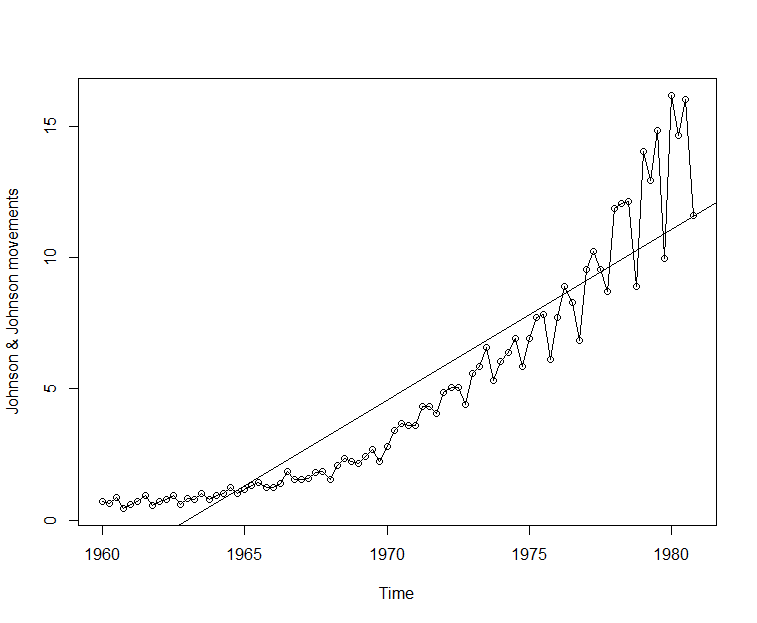
\includegraphics[width=0.9\linewidth]{../Beamer/linearreg}
\end{figure}

It is apparent that the estimated trend line obtained via simple linear regression does not
quite capture the trend of the data and better models will be needed. 					

\section{Preliminaries}
\subsection{White noise and Moving average}
White noise describes each element in a series is a random draw from a population of mean 0 and constant variance. A moving-average model is conceptually a linear regression of the current value of the series against current and previous (unobserved) white noise error terms or random shocks. The random shocks at each point are assumed to be mutually independent and to come from the same distribution, typically a normal distribution, with location at zero and constant scale. 


A simple kind of generated series might be a collection of uncorrelated random variables, $ \epsilon_t $ with mean $ 0 $ and finite variance $ \sigma^2 $. The time series generated from uncorrelated variables is used as a model for noise in some applications, where it is called white noise. \\
A particularly useful white noise series is Gaussian white noise, wherein the $ \epsilon_t $ are independent normal random variables, with mean $ 0 $ and variance $ \sigma^2 $.  
The below figure shows on the upper panel a collection of 500 such random variables, with $ \sigma_\epsilon^{2} = 1$. Replacing the white noise by a moving average that smooths the series results in the bottom figure. This can be done by replacing $ \epsilon_t $ by an average
of its current value and its immediate neighbours in the past and future ie,

\begin{equation*}
v_t = \frac{1}{5} (\epsilon_{t-2}+\epsilon_{t-1}+ \epsilon_t + \epsilon_{t+1}+ \epsilon_{t+2})
\end{equation*}

\begin{figure}
	[h]
	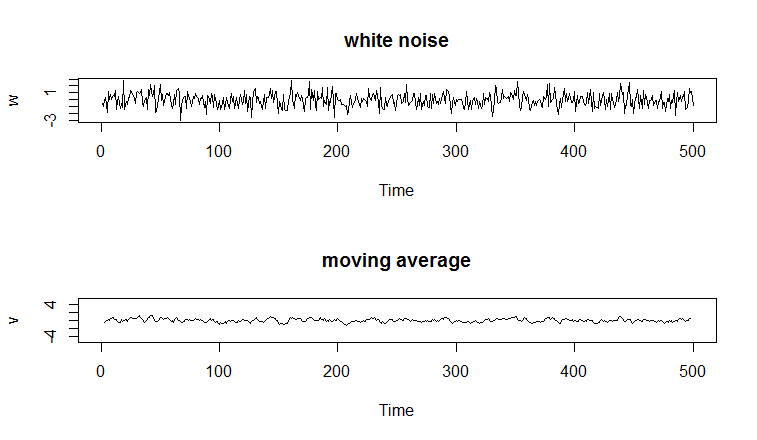
\includegraphics[width=0.9\linewidth]{../Beamer/whitenoise_ma_5}
	\caption{}
	\label{}
\end{figure}

These are plotted in R using the following commands. 

\begin{lstlisting}
w = rnorm(500,0,1)  # 500 samples that follow N(0,1)
v = filter(w, sides=2, rep(1/5,5))  # computing moving average. As shown in vt.
plot.ts(w, main="white noise")
plot.ts(v, ylim=c(-5,5), main="moving average")
\end{lstlisting}

\subsection{Stationary Series.}
A series is stationary when the mean and variance do not change over time and the process does not have trends. Modelling a time series (ARMA) model requires stationarity. Also for an \textit{Auto Correlation function} (ACF) to make sense, the series must be a \textit{weakly stationary series}. This means that the autocorrelation for any particular lag is the same regardless of where we are in time. \\

A series is said to be weakly stationary if it satisfies the following conditions;\\
\begin{itemize}
\item The mean $ E(x_t) $ is same for all $ t $
\item The variance  of $ (x_t) $ is same for all $ t $	
\item The covariance and the correlation between $ x_t $ and $ x_{t-h} $ is the same for all $ t $.
\end{itemize}

\textbf{Differencing:} One of the ways we can address the issue of stationariness us by \textit{differencing}. It involves two steps. 
\begin{itemize}
	\item Remove unequal variances. We do this using log of the series. 
	\item We need to address the trend component. We do this by taking \textit{difference} of the series.
	\item Differenced variable: $ \Delta x_t = x_t - x_{t-1}$
\end{itemize} 

This can be done using \textit{diff(log(JohnsonJohnson))} in R. So the Johnson Johnson stock which was a non stationary series can be transformed as follows. 

\begin{figure}
[h]
	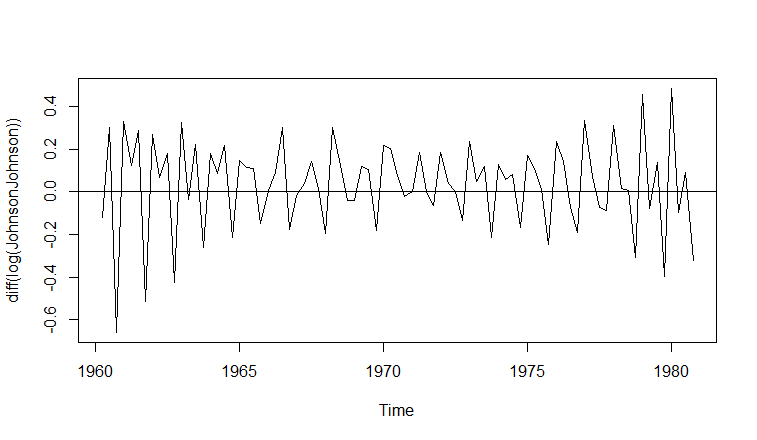
\includegraphics[width=0.9\linewidth]{difflog}
\end{figure}

\subsection{Augmented Dickey–Fuller test}
Augmented Dickey–Fuller test \textbf{(ADF)} tests the null hypothesis of whether a unit root is present in a time series sample. The alternative hypothesis is usually stationarity or trend-stationarity. 

The testing procedure for the ADF test is applied to the AR(1) model;

\begin{equation}
x_t = \rho x_{t-1} + e_t
\end{equation}

\begin{align*}
x_t &: \text{is the variable of interest}\\
\rho &: \text{coefficient on a time trend} \\
e_t &: \text{error term}
\end{align*}

A unit root is present if $ \rho=1 $. The model would be non-stationary in this case. We rewrite Equation(2) as, 

\begin{align*}
x_t &= \rho x_{t-1} +\epsilon_t \\
x_t - x_{t-1} &= \rho x_{t-1} -x_{t-1} +\epsilon_t \\
\delta x_t &= (\rho-1) y_{t-1} +\epsilon_t\\
\delta x_t &= \gamma y_{t-1} +\epsilon_t\\
\end{align*}

If $ \gamma = 0 $ then we have $ \rho=1 $, then it means $ x_t = x_{t-1} +\epsilon_t $. Which is nothing but a \textit{random walk}. So we can say $ x_t $ is not stationary. We therefore obtain the below hypothesis. \\

\textbf{Estimation:} We estimate if null-hypothesis is not rejected, then $ x_t $ is not stationary. \\

Testing ADF on our data JohnsonJohnson, in R, we have the following result. 

\begin{figure}
[h]
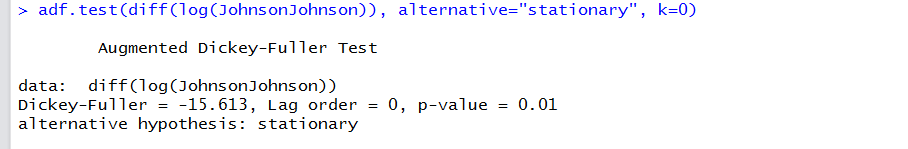
\includegraphics[width=1\linewidth]{ADFtest}
\end{figure}

\textbf{Note:} A small $ p $ value ($ \leq 0.05 $) indicates strong evidence against the null hypothesis, so you reject the null hypothesis. 

\subsection{Autocorrelation function (ACF)}
The coefficient of correlation between two values in a time series is called the autocorrelation function (ACF) For example the ACF for a time series $ x_t $ is given by:
\begin{equation*}
Corr(x_t,x_{t-k}) 
\end{equation*}

This value of $ k $ is the time gap being considered and is called the lag. A lag 1 autocorrelation (i.e., $ k = 1 $ in the above) is the correlation between values that are one time period apart. More generally, a lag $ k $ autocorrelation is the correlation between values that are $ k $ time periods apart.  The ACF is a way to measure the linear relationship between an observation at time $ t $ and the observations at previous times. If we assume an AR(k) model, then we may wish to only measure the association between $ x_t $ and $ x_{t-k} $ and filter out the linear influence of the random variables that lie in between (ie. $ x_{t-1},x_{t-2}......x_{t-k}  $). 

Theoretically, the autocorrelation between $ x_t $ and $ x_{t-k} $ is, 	

\begin{equation*} 
ACF(k) = \frac{\text{Covariance}(x_t,  x_{t-k})}{\sigma_{{x_t}}. \sigma_{x_{t-k}}}  = \frac{\text{Covariance}(x_t, x_{t-k})}{\text{Variance}(x_t)}
\end{equation*}

We plot the ACF of our Johnson and Johnson stock and see the difference between the stationary and non stationary series. 

\begin{figure}
[h]	
	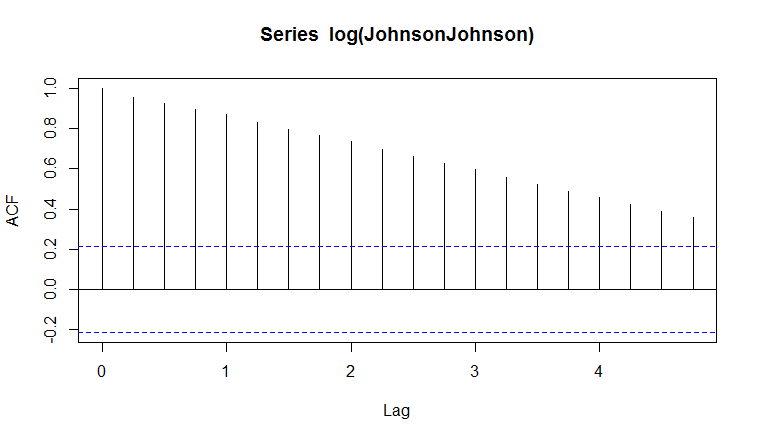
\includegraphics[width=0.475\textwidth]{../Beamer/ACF_log}
	\hfill
	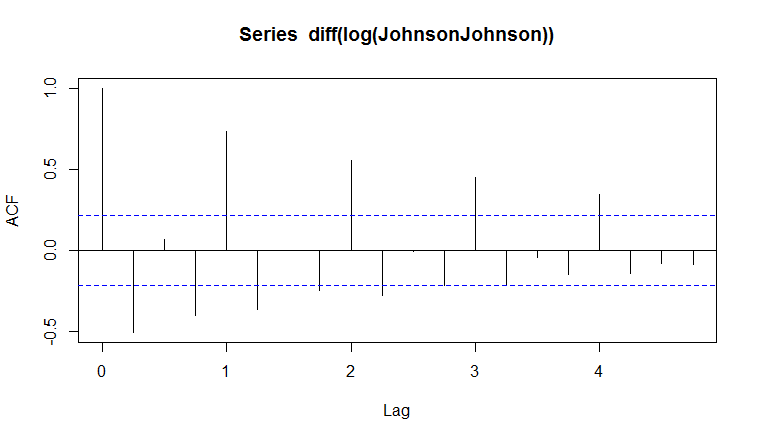
\includegraphics[width=0.475\textwidth]{../Beamer/ACF_logdiff}
	\caption{ACF of a non-stationary  vs stationary series}
	\label{fig}
\end{figure}

The ACF is “decaying”, or decreasing, very slowly, and remains well above the significance range (dotted blue lines). This is indicative of a non-stationary series. Refer Figure \ref{fig}\\
	
On the other hand ACF of a stationary series shows exponential decay. This is indicative of a stationary series.

\subsection{Partial Autocorrelation function (PACF)}
PACF is a simple correlation between $ x_t $ and $ x_{t-k} $, minus the part explained by the intervening lags. 	

\begin{equation*}
\rho_k = Corr (x_t - E(x_t |x_{t-1} .... x_{t-k+1}),x_{t-k})
\end{equation*}

where; \\
$ E(x_t |x_{t-1} .... x_{t-k+1}) $ is the minimum squared error predictor. 

The 2nd order (lag) partial autocorrelation is; 

\begin{equation}
\frac{\text{Covariance}(x_t, x_{t-2}| x_{t-1})}{\sqrt{\text{Variance}(x_t|x_{t-1})\text{Variance}(x_{t-2}|x_{t-1})}}
\end{equation}

We visualize using this PACF Plot. The plot indicates that the PACF cuts off past the order of the model. 

\begin{figure}
	[h]
	\centering
	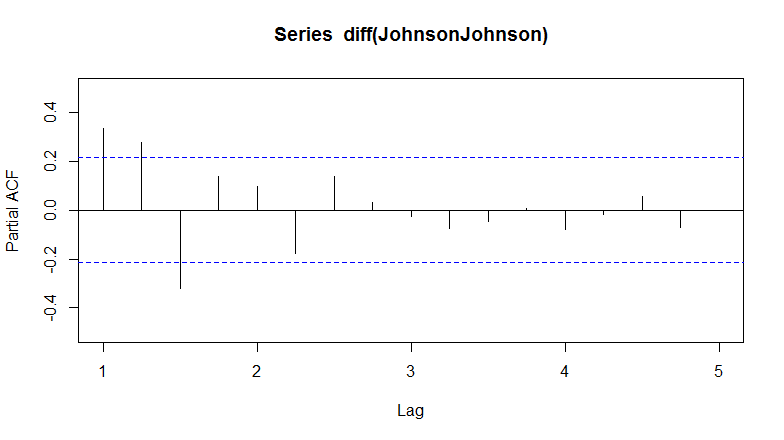
\includegraphics[width=0.8\linewidth]{pacf_jj}
\end{figure}

\section{ARIMA models}
\subsection{Introduction}
Linear models where built based on classical regression theory for exploiting the associations
indicated by large values of the ACF. The time domain, or regression, are appropriate when we are dealing with possibly nonstationary, shorter time series. In addition, if the emphasis is on
forecasting future values, then the problem is easily treated as a regression problem. 

The introduction of correlation as a phenomenon that may be generated through lagged linear relations leads to proposing the autoregressive \textbf{(AR)} and autoregressive moving average \textbf{(ARMA)} models. Adding nonstationary models to the mix leads to the autoregressive integrated moving average \textbf{(ARIMA)}. 

In the time series case, it is desirable to allow the dependent variable to be influenced by the past values and possibly by its own past values. If the present can be modelled in terms of only the past values of the independent inputs, we have the prospect that forecasting will be possible.

\subsection{First-order Autoregression Model (AR(1))}
A time series is a sequence of measurements of the same variable(s) made over time. Usually the measurements are made at evenly spaced times - for example, monthly or yearly. Let us first consider the problem in which we have a $ x $-variable measured as a time series. As an example, we might have $ x $ a measure of global temperature, with measurements observed each year. 
To emphasize that we have measured values over time, we use "t" as a subscript, i.e $ x_t $ means $ x $ measured in time period $ t $. 

In this model the value of $ x $ at time $ t $ is a linear function of the value of $ x $ at time $ t-1 $

\begin{equation*}  
x_{t}=\beta_{0}+\beta_{1}x_{t-1}+\epsilon_{t}  
\end{equation*}

Assumptions:

\begin{itemize}
\item $ \epsilon_t \overset{iid}{\sim} N(0, \sigma^2) $ ie errors are independently distributed with a normal distribution that has mean 0 and constant variance.	
\item Properties of the errors $ \epsilon_t $ are independent of $ x_t $.
\item The series $ x_1,  x_2,  ...  $ is (weakly) stationary.
\end{itemize}

The order of an autoregression is the number of immediately preceding values in the series that are used to predict the value at the present time. So, the preceding model is a first-order autoregression, written as AR(1). 

If we want to predict $ x $ this year $ x_t $ using measurements of global temperature in the previous two years $ (x_{t-1}, x_{t-2}) $, then the autoregressive model for doing so would be:

\begin{equation*}  
x_{t}=\beta_{0}+\beta_{1}x_{t-1}+\beta_{2}x_{t-2}+\epsilon_{t}  
\end{equation*}

This model is a second-order autoregression, written as AR(2), since the value at time $ t $ is predicted from the values at times $ t-1 $ and $ t-2 $. \\

An autoregressive model of order $ p $, AR(p), is of the form;  

\begin{equation}  
x_{t}=\beta_{0}+\beta_{1}x_{t-1}+\beta_{2}x_{t-2}+ .... \beta_{p}x_{t-p}+ \epsilon_{t}  
\end{equation}

The mean of $ x_t $ is zero. If the mean $ \mu $ of $ x_t $ is not zero, we replace $ x_t $ by $ x_{t} - \mu $ in above and write as; 

\begin{equation}  
x_{t}=\alpha + \beta_{1}x_{t-1}+\beta_{2}x_{t-2}+ .... \beta_{p}x_{t-p}+ \epsilon_{t}  
\end{equation}

where $ \alpha = \mu(1-\beta_1.....- \beta_p) $. 

We note that this equation is similar to the regression model of (1) and hence the term \textit{auto (or self) regression.}\\


\begin{exmp}{Sample path of an AR(1) process}\\
Lets see a time plot of two AR(1) processes. One with $ \beta = 0.9 $ and another with $ \beta = -0.9 $. The first case shows observations close together in time are positively correlated with each other. It means observations at contiguous time points will tend to be close in value to each other; this fact shows up a very smooth sample path for $ x_t $. \\
For the second case $ \beta = -0.9 $ the result means that observations at contiguous time points are negatively correlated but observations two time points apart are positively correlated. This shows up in the figure where for example, if an observation $ x_t $ is positive the next observation $ x_{t+1} $ is typically negative and the next $ x_{t+2} $ is positive. Thus, in this case, the sample path is very \textit{choppy}.
\end{exmp}


\begin{figure}
[h]
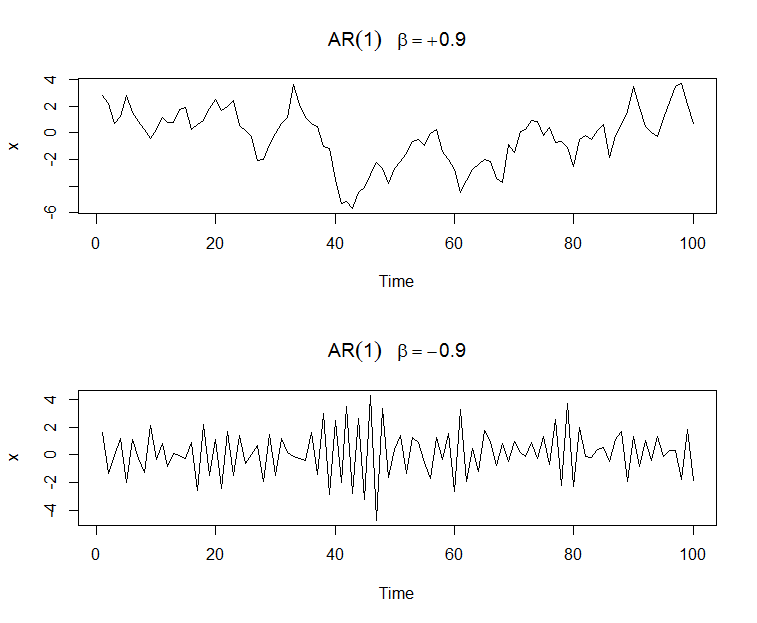
\includegraphics[width=0.9\linewidth]{AR(1)}
\end{figure}

\begin{paragraph}{ACF for AR(1)}
For an AR(1) model, the ACF is ACF(h) = $ \rho_k = \beta^k $. We say this function tails off as in Figure \ref{ACF_ar1}.   
\end{paragraph}


\begin{figure}
[h]
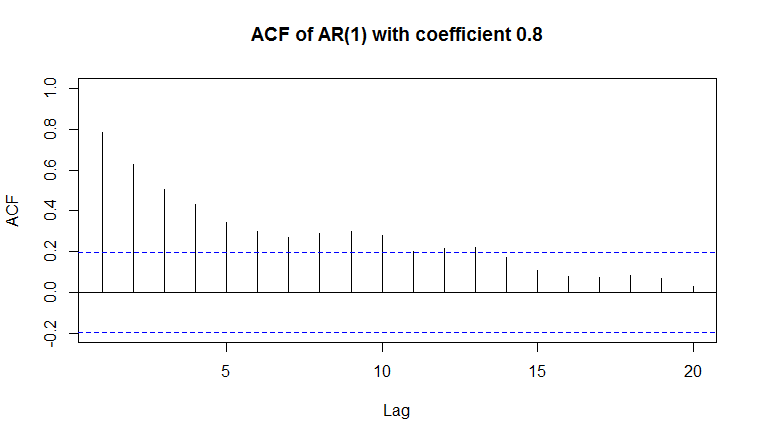
\includegraphics[width=0.9\linewidth]{../Beamer/ACF_ar1}
\label{ACF_ar1}
\caption{ACF for AR(1)}
\end{figure}

We plot this using the below R codes. 

\begin{lstlisting}
ar <- arima.sim(model=list(ar=.8), n=100)   # Simulating an AR process. 
plot(ar)

#Plotting ACF of an AR with coefficient 0.8 
acf(ar,20,xlim=c(1,20),main="ACF of AR(1) with coefficient 0.8")   
\end{lstlisting}

\begin{paragraph}{PACF for AR(1)}
Now we look at PACF for AR(1) process. Refer Figure 4: PACF for AR(1). As we see, the first spike is the correlation between $ x_t $ and $ x_{t-1}  $ which is $ 0.8. $. What is the correlation between $ x_t $ and $ x_{t-2} $ ? Nothing. Since everything comes from the first lag. Once we come from the first lag there are no more residual correlations. That is why we say it \textit{cuts off.}. \\
If you have an AR(2) process, then you will have 2 lags and then everything else will cut off. Ref \ref{Pacf}
\end{paragraph}

\begin{figure}
[h]
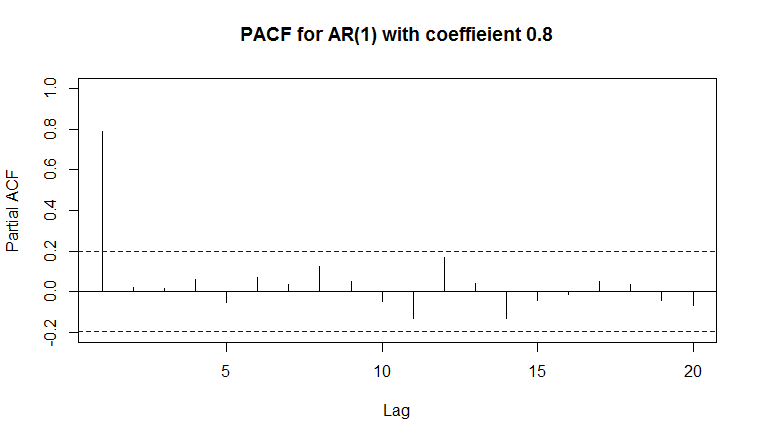
\includegraphics[width=0.9\linewidth]{ar1_pacf}
\label{Pacf}
\caption{PACF for AR(1)}
\end{figure}


\begin{lstlisting}
pacf(ar,20,ylim=c(-.2,1),main="PACF for AR(1) with coeffieient 0.8")
\end{lstlisting}

\subsection{Moving Average (MA) model}
A moving average term in a time series model is a past error (multiplied by a coefficient). 
In time series analysis, the moving-average (MA) model is a common approach for modeling univariate time series. The moving-average model specifies that the output variable depends linearly on the current and various past values of a stochastic (imperfectly predictable) term. Together with the autoregressive (AR) model, the moving-average model is a special case and key component of the more general ARMA and ARIMA models of time series, which have a more complicated stochastic structure. 

A first order moving average model, denoted by MA(1) is	given by; 
\begin{equation*}
x_t =\mu + \epsilon_t +\theta_1\epsilon_{t-1}
\end{equation*}

and the \textit{qth} order moving average model \textbf{MA(q)} is given by; 

\begin{equation*}
x_t = \epsilon_t +\theta_1\epsilon_{t-1}+\theta_2\epsilon_{t-2}+\dots + \theta_q\epsilon_{t-q}
\end{equation*}

where;\\
$ \mu $ is the mean of the series. \\
$ \,\theta_1,\theta_2....\theta_q $ are the parameters of the model \\
value $ q $ is the order of the MA model. 

Moving average (MA) models account for the possibility of a relationship between a variable
and the residuals from previous periods. Notice that here there are no $ x_{t-1}, x_{t-1} ... $ terms. MA model is all about the residuals unlike the AR which is about the lags of the variable itself. \\

\begin{exmp}{Sample path of an MA(1) process}\\
When for e.g $ \theta = 0.7 $,  $ x_t $ and $ x_{t-1} $ are positively correlated and when $ \theta = - 0.7 $, they are negatively correlated. Refer Figure 5: MA(1) path. The plot shows that the series is \textit{smoother} when $ \theta = 0.7 $. 
\end{exmp}

\begin{figure}
\centering
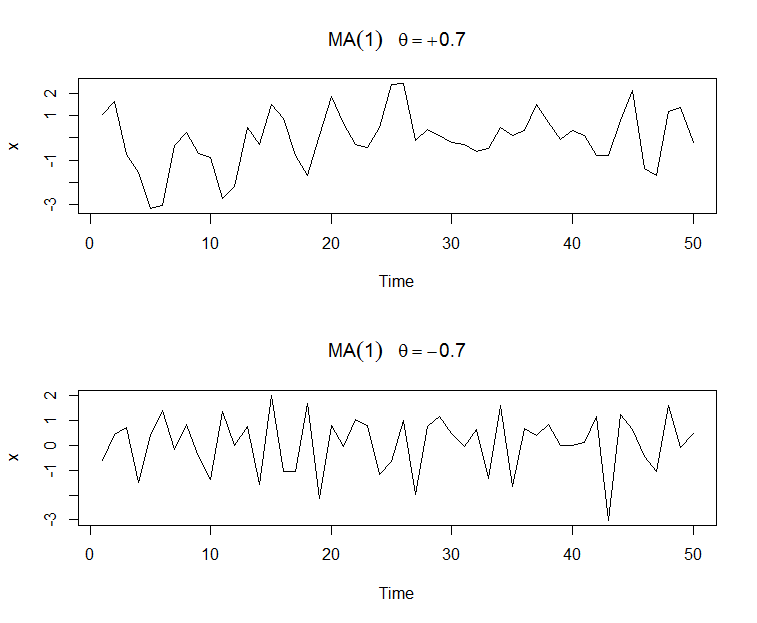
\includegraphics[width=0.9\linewidth]{ma1}
\label{ma1}
\caption{MA(1) path}
\end{figure}

We use this code format to drive the results in R. 
\begin{lstlisting}
plot(arima.sim(list(order=c(0,0,1), ma=.7), n=50),
	 ylab="x",main=(expression(MA(1)~~~theta==+.7)))
plot(arima.sim(list(order=c(0,0,1), ma=-.7), n=50),
	 ylab="x",main=(expression(MA(1)~~~theta==-.7)))
\end{lstlisting}
	
	
\subsection{ARMA Model}	
We may have to use a relatively long AR or MA model to capture the complex structure of time series. This sometimes is undesirable as we usually want to fit stingy models i.e a model with relatively few unknown parameters.  To achieve this goal we combine the AR and MA parts to form a ARMA (\textit{Autoregressive Moving Average model.)}

\begin{paragraph}{Definition:}
A time series $ {x_t: t = 0,\pm 1, \pm 2,..} $ is ARMA(p,q) if it is stationary and 

\begin{equation}
x_t = \phi_1 x_{t-1} +....\phi_p x_{t-p} +w_t + \theta_1 w_{t-1} +\theta_q w_{t-q}
\end{equation}
\end{paragraph}

The parameters $ p $ and $ q $ are called the autoregressive and the moving average orders, respectively. If $ x_t $ has a nonzero mean $ \mu $, we set $ \alpha = \mu(1-\phi_1....-\phi_p) $ and write the model as ;

\begin{equation*}
x_t = \alpha + \phi_1 x_{t-1} +....\phi_p x_{t-p} +w_t + \theta_1 w_{t-1} +\theta_q w_{t-q}
\end{equation*}

As previously noted, when $ q = 0 $, the model is called an autoregressive model of order $ p $, AR(p), and when $ p = 0 $, the model is called a moving average model of order $ q $, MA(q).
	
The ARMA(p,q) model in (4) can then be written in concise form as,
\begin{equation}
\phi(B) x_t = \theta(B) w_t
\end{equation}

\newpage
\begin{thebibliography}{9}
	\bibitem{} 
	Robert H. Shumway , David S. Stoffer
	\newblock {\em Time Series analysis and its applications}
	
	\bibitem{}
	Rob J Hyndman, George Athana­sopou­lo
	\newblock {\em Forecasting: Principles and practice}
	
	\bibitem{}
	The Pennsylvania State University - STAT 510 - Applied Time Series analysis \\
	\newblock \url{https://onlinecourses.science.psu.edu/stat510/}	
	
	\bibitem{}
	R Documentation
	\newblock \url{https://www.rdocumentation.org/}	 	
	
\end{thebibliography}
		
	
\end{document}